% !TEX root = ../../../semexp-thesis.tex

\section{Tool Support}
\label{sec:semtex/tools}

Developing semantic applications (i.e., programs that rely on semantic technologies) presents particular challenges to programmers, including nondeterministic behavior, latencies, and cost of language models.

First, language models behave \emph{nondeterministically} in many settings, which can impede testing.
In particular, generative LLMs exhibit characteristics of a chaotic system, meaning that small changes in the provided input might cause large changes in their outputs.
For example, if the user phrases the same question using slightly different words, an agent might interpret the task very differently and fail to solve it appropriately.
Thus, the behavior of LLMs is often poorly predictable.

Second, requesting language models to process large amounts of information can involve notable \emph{latencies}, which result from the intrinsic speed of models and possible rate limits of APIs.
For example, embedding or describing all methods in a typical Squeak image using contemporary OpenAI models might take between five and ten minutes~(see \cref{sec:discussion/somewhere}).
These delays can reduce the experience of temporal immediacy for programmers who are prototyping or testing semantic applications.

Third, \emph{pecuniary costs} often arise when using cloud models.
Sending a single message to an object or evaluating a simple script during prototyping might suddenly involve expenses of several (US) cents or sometimes even dollars.
These expenses are largely unexpected, invisible, and difficult to track.
This can result not only in unintended invoices but also overcautiousness in developers, forming a new kind of psychological barrier to the experienced immediacy of programmers.

Through the \semtex framework, we provide different tools for addressing these challenges and thus improving the development experience of semantic-application programmers:
a \emph{conversation editor} for prototyping generative agents, a \emph{mocking provider} for replacing slow and expensive language models, and means for \emph{price estimation} and \emph{expense watching}.

\subsection{Conversation Editor}
\label{sec:semtex/tools/editor}

The \emph{conversation editor} is a graphical tool through that programmers can prototype and debug generative agents.
It allows programmers to inspect and modify all parts of a conversation such as messages, functions, and function calls using a text-based WYSIWYG\footnote{WYSIWYG: What you see is what you get.} interface.

For example, programmers can engage in prompt engineering by drafting different versions of system instructions and function specification and comparing their effect (by duplicating the conversation window using the eponymous Morphic halo handle in Squeak).
Moreover, they can simulate the behavior of certain function calls or former assistant replies without implementing them.
Thus, the conversation editor allows programmers to test agents and explore the efficacy of different prompts%
\footnote{%
	Similar possibilities are offered by several other tools such as the \emph{OpenAI chat playground} (\url{https://platform.openai.com/playground/chat}).
	However, existing tools are typically not integrated into the live programming system, which impedes prototyping, since programmers need to connect language models with other artifacts and logic.
	In addition, our conversation editor can also be used for post-mortem-debugging and exploring actual conversations from a semantic application.
}%
.

\begin{figure}
	\centering
	% todo: two images next to each other!
	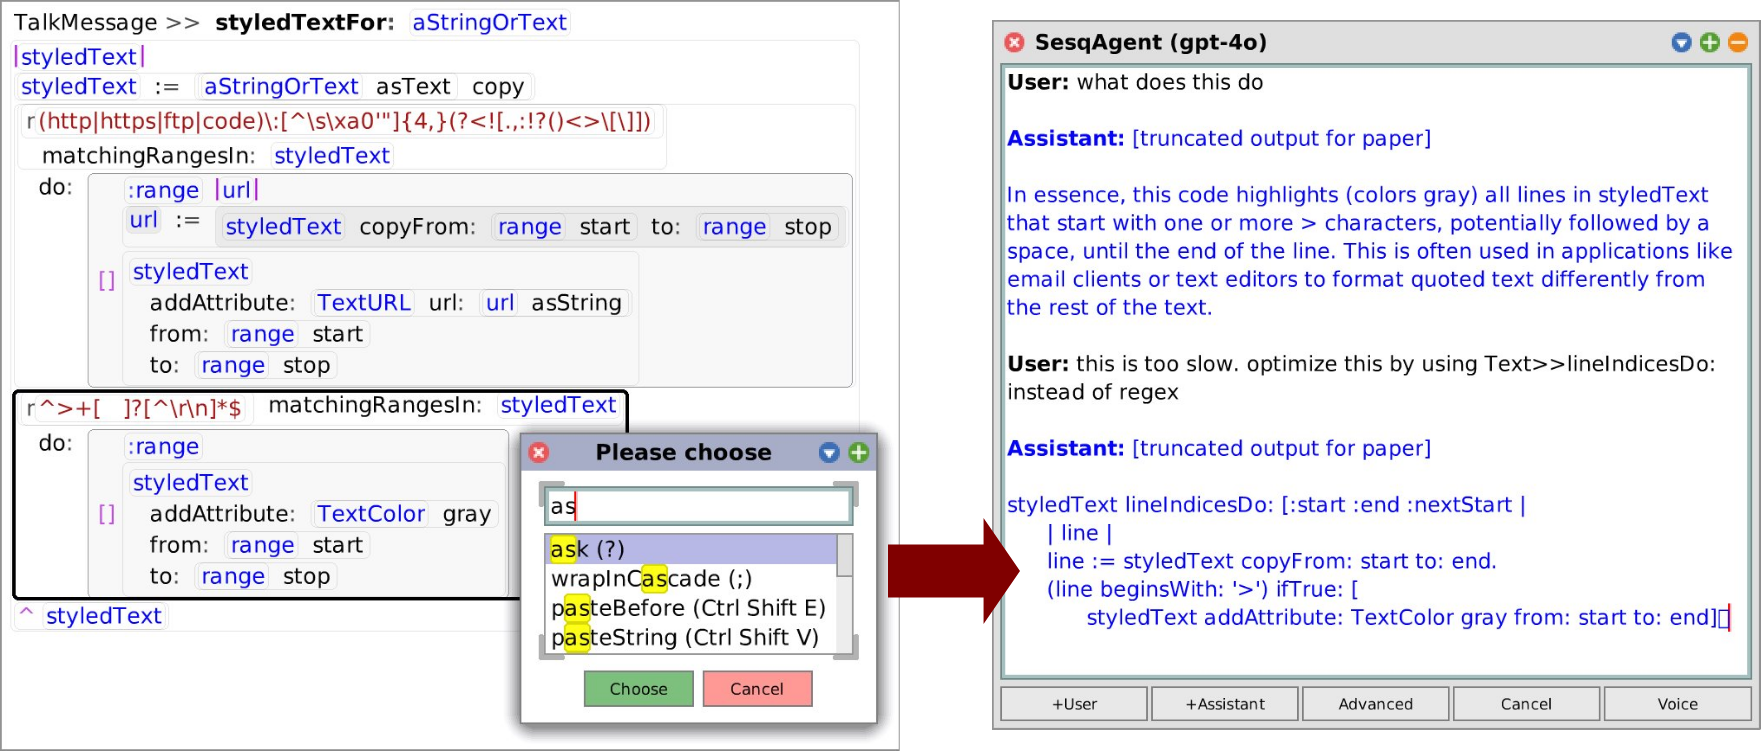
\includegraphics[width=\textwidth]{a_semtex/tools/editor.png}
	\caption[TODO]{
		TODO
	}
	\label{fig:semtex/tools/editor}
\end{figure}

The GUI of the conversation editor provides two modes~(\cref{fig:semtex/tools/editor}):
the \emph{default mode} only shows user and assistant messages, whereas the \emph{advanced mode} also provides read and write access to system messages as well as function specifications, function calls, and function results.
So, while the advanced mode is intended for prototyping and debugging, the former mode functions as an interface for end users.
The conversation editor also constitutes a composable UI component that can be reused by semantic applications such as our conversational prototype for the semantic workspace~(see \cref{sec:implementation/conversations}).

\subsection{Mocking Provider}
\label{sec:semtex/tools/mocking}

\semtex implements a mocking provider with different \emph{mocking models} that simulate the behavior of real language models through simple heuristics.
The \code{MockingConversationModel} answers a static assistant message for each request (which can be adjusted through parameters in the \code{SemanticConversationConfig}).
The \code{MockingEmbeddingModel} embeds each document as a small vector based on the term frequencies of a short hard-coded list of words.

By temporarily using mocking models, programmers can ensure the deterministic behavior of semantic application while testing them or developing other parts of a system.
Finally, they can avoid additional latencies or costs.

\subsection{Price Estimation and Expense Watching}
\label{sec:semtex/tools/pricing}

To facilitate planning of expenses, model providers offer means for \emph{estimating} the prices of requests before actually submitting them to an API.
Additionally, they \emph{log} the expenses from submitted requests.
For this, they use a combination of usage statistics returned from API responses (such as the number of processed tokens) and local (approximating) cost models.

This allows for the construction of \emph{expense watchers} that display the expenses for semantic operations in single tools such as the conversation editor or in the global system~(\cref{fig:semtex/tools/pricing/expense_watchers})%
\footnote{%
	This resembles common usage dashboards of cloud services such as OpenAI (\url{https://platform.openai.com/usage}).
	However, expense watchers in \semtex detail costs with a finer granularity and improve visibility through direct integration into the programming system.
}%
.
Thus, programmers gain improved trust and transparency regarding pecuniary costs of language models.

\begin{figure}
	\centering
	% todo: two images next to each other!
	\includegraphics[width=\textwidth]{a_semtex/tools/pricing/expense_watchers.png}
	\caption[TODO]{
		TODO
	}
	\label{fig:semtex/tools/pricing/expense_watchers}
\end{figure}
